\section{Mạng điện thoại}
Mạng điện thoại, là mạng cố định liên kết không dây, truyền các cuộc gọi điện thoại, là một trong những mạng truyền thông lâu đời nhất vẫn được sử dụng (mặc dù mạng bưu chính chắc cũ hơn), chủ yếu được nghiên cứu bởi các nhà nghiên cứu mạng lý thuyết, vì thường thiếu dữ liệu tốt về cấu trúc của nó. Cấu trúc của mạng điện thoại đã được biết, nhưng dữ liệu phần lớn được các công ty điện thoại sở hữu, chúng không được chia sẻ công khai với cộng đồng nghiên cứu theo cách giống như dữ liệu Internet. Chúng tôi hy vọng rằng tình trạng này sẽ thay đổi, mặc dù vấn đề có thể trở nên khó khăn trong tương lai không xa, vì các công ty điện thoại đang gửi một lượng lưu lượng thoại ngày càng tăng qua Internet thay vì qua các đường dây điện thoại chuyên dụng, và có thể không lâu nữa hai mạng hợp nhất thành một.\par
Một số nguyên tắc hoạt động chung của mạng điện thoại khá là rõ ràng. Ngược lại với Internet, mạng điện thoại truyền thống không phải là chuyển mạch gói. Tín hiệu được gửi qua mạng điện thoại không được phân tách và gửi dưới dạng các gói riêng biệt. Thay vào đó, mạng điện thoại được chuyển mạch kênh, nghĩa là công ty điện thoại có sẵn đường dây hoặc mạch để thực hiện các cuộc gọi điện thoại giữa các điểm khác nhau. Trong những ngày đầu tiên của các hệ thống điện thoại ở Hoa Kỳ và Châu Âu, các đường dây thực sự riêng lẻ, mỗi đường dây là một cuộc gọi, tăng khả năng của mạng, gọi nhiều cuộc gọi hơn là đặt nhiều dây hơn. Tuy nhiên, từ đầu thế kỷ XX, các công ty điện thoại đã sử dụng các kỹ thuật để ghép tín hiệu điện thoại, tức là nhiều cuộc gọi cùng một dây. Cáp điện thoại trong một nhà thường chỉ thực hiện một cuộc gọi mỗi lần, mặc dù điều đó đã thay đổi trong những năm gần đây vì công nghệ mới đã giúp các hộ gia đình có thể có nhiều hơn một số điện thoại và thực hiện nhiều cuộc gọi cùng một lúc.\par
\begin{figure}[ht]
\centering
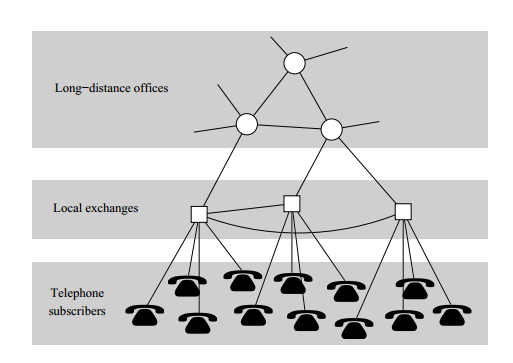
\includegraphics[width=0.5\textwidth]{res/h24.png}
\caption{Sơ đồ cấu trúc ba tầng của mạng điện thoại truyền thống}
\label{fig:h24}
\end{figure}\par
Các hình thức cơ bản của mạng điện thoại là tương đối đơn giản. Hầu hết các quốc gia có mạng điện thoại cố định sử dụng thiết kế ba tầng. Các thuê bao điện thoại cá nhân được kết nối qua các đường dây điện thoại với các tổng đài điện thoại địa phương, sau đó được kết nối qua các đường dây chia sẻ với các văn phòng đường dài (Long-distance offices), đôi khi còn được gọi là văn phòng chuyển mạch (toll-switching offices). Các văn phòng đường dài được kết nối với nhau bằng các đường trung kế (Further trunk lines).(Hình \ref{fig:h24}). Cấu trúc này khá giống với cấu trúc của Internet (Hình \ref{fig:h21}), mặc dù các nguyên tắc hoạt động cơ bản của hai mạng khá khác nhau.\par
Cấu trúc liên kết ba cấp của mạng điện thoại được thiết kế để khai thác các cuộc gọi điện thoại ở hầu hết các địa phương, có nghĩa là chúng kết nối các thuê bao trong cùng thị trấn hoặc khu vực. Các cuộc điện thoại giữa các thuê bao được kết nối cùng địa phương có thể được xử lý chỉ bằng trao đổi mà không cần sử dụng bất kỳ đường trung kế nào cả. Các cuộc gọi như vậy thường được gọi là các cuộc gọi nội hạt (local calls) , trong khi các cuộc gọi đi qua các đường trung kế được gọi là các cuộc gọi đường dài. \par
Mạng điện thoại đã có cấu trúc tương tự như vậy trong hàng trăm năm qua và vẫn còn cho đến ngày nay, chỉ là nhiều chi tiết về cách thức hoạt động của mạng đã thay đổi. Đặc biệt, ở cấp trung kế, một số mạng điện thoại không còn được chuyển mạch kênh. Thay vào đó, giờ đây chúng là các mạng chuyển mạch gói kỹ thuật số hoạt động theo cách khác với Internet, với các cuộc gọi thoại được số hóa, chia thành các gói và truyền qua các liên kết cáp quang. Tuy nhiên, về mặt hình học và cấu trúc liên kết, cấu trúc của mạng điện thoại vẫn giống như trước đây, bị chi phối bởi những hạn chế về địa lý và xu hướng mọi người nói chuyện thường xuyên hơn với những người trong vùng lân cận hơn là với những người ở xa.\par

\section{Lưới điện}
Một mạng lưới điện, trong bối cảnh này, là mạng lưới các đường dây điện cao thế cung cấp vận chuyển điện đường dài trong các quốc gia. Đường dây cung cấp điện cục bộ có điện áp thấp thường được loại trừ. Các đỉnh trong lưới điện tương ứng với các trạm phát và trạm chuyển mạch, và các cạnh tương ứng với các đường dây cao thế. Cấu trúc liên kết của lưới điện không khó để xác định. Các mạng được giám sát bởi một cơ quan duy nhất và bản đồ lưới được hoàn chỉnh sẵn. Thật vậy, dữ liệu về lưới điện rất toàn diện (cũng như các mạng liên quan đến năng lượng khác như đường ống dẫn dầu và khí đốt) có sẵn từ các nhà xuất bản chuyên nghiệp, trên giấy hoặc dưới dạng điện tử cho ai sẵn sàng trả tiền cho chúng.\par
Ta học được nhiều điều thú vị bằng cách nhìn vào cấu trúc của lưới điện. Giống như Internet, lưới điện có khía cạnh không gian, mỗi đỉnh riêng lẻ là một vị trí ở đâu đó trên toàn cầu và sự phân bố của chúng trong không gian rất thú vị từ quan điểm địa lý, xã hội và kinh tế. Thống kê cả về địa lý và cấu trúc liên kết có thể cung cấp cái nhìn sâu sắc về các hạn chế chi phối hình dạng và sự tăng trưởng của lưới điện. Các lưới điện cũng hiển thị một số hiện tượng bất thường, chẳng hạn như sự cố xếp tầng, có thể dẫn đến kết quả tìm được luật của quy mô mất điện.\par
Lưới điện là hệ thống rất phức tạp. Dòng điện không chỉ bị chi phối bởi các định luật vật lý đơn giản mà còn bởi sự điều khiển chính xác và chi tiết các pha và điện áp trên các đường truyền, được theo dõi và điều chỉnh theo thời gian nhanh bởi các hệ thống máy tính tinh vi và thời gian chậm hơn bởi con người. Nó chỉ ra rằng sự cố mất điện và các hiện tượng lưới điện khác bị ảnh hưởng tương đối ít bởi cấu trúc liên kết thô của mạng mà phần nhiều là bởi các hoạt động của nhà điều hành và thiết kế phần mềm.\par

\section{Mạng vận tải}
Một lượng công việc đã được thực hiện trên cấu trúc của các mạng lưới giao thông như đường hàng không, đường bộ và đường sắt. Cấu trúc của các mạng này thường không khó xác định, mặc dù việc biên dịch dữ liệu có thể tốn nhiều công sức. Mạng lưới hàng không có thể được xây dựng từ thời gian biểu của hãng hàng không, mạng lưới đường bộ và đường sắt thì từ bản đồ. Phần mềm hệ thống thông tin địa lý (Geographic information systems -GIS) có thể hữu ích để tăng tốc độ tổng hợp dữ liệu, và cũng có nhiều nguồn tài nguyên trực tuyến cung cấp thông tin hữu ích như vĩ độ và kinh độ của các sân bay.\par
Một trong những ví dụ sớm nhất về một nghiên cứu về mạng lưới giao thông là nghiên cứu của Forge về vận tải đường thủy trên các dòng sông của Nga vào thời Trung cổ. Cũng có một phong trào giữa các nhà địa lý trong những năm 1960 và 70 để nghiên cứu mạng lưới đường bộ và đường sắt, đặc biệt tập trung vào sự tương tác giữa kinh tế và cấu trúc vật lý. Cái tên nổi bật nhất trong phong trào này là của Karel Kansky, và cuốn sách về mạng lưới giao thông của ông là tác phẩm tiêu biểu.\par
Gần đây, một số tác giả đã tạo ra các nghiên cứu áp dụng các ý tưởng phân tích mạng mới cho mạng lưới đường bộ, đường sắt và đường hàng không. Trong hầu hết các mạng được nghiên cứu, các đỉnh đại diện cho các vị trí địa lý và các tuyến đường cạnh giữa chúng. Ví dụ, trong các nghiên cứu về mạng lưới đường bộ, các đỉnh thường đại diện cho giao lộ đường và các đường biên. Nghiên cứu của Sen, mạng lưới đường sắt của Ấn Độ cung cấp một điều thú vị, Sen lập luận rằng, trong bối cảnh du lịch đường sắt, điều quan trọng nhất đối với hầu hết mọi người là liệu có một chuyến tàu trực tiếp đến đích của họ hay không, nếu không, họ sẽ phải đi bao nhiêu chuyến tàu để đến đó. Mọi người không quan tâm quá nhiều đến việc có bao nhiêu điểm dừng trên đường đi, miễn là họ không phải đổi tàu. Do đó, Sen lập luận, một đại diện mạng hữu ích trong trường hợp di chuyển bằng đường sắt là hai đỉnh đại diện vị trí, và hai đỉnh đó được nối với nhau bởi một cạnh nếu một đoàn tàu chạy giữa chúng. Số cạnh bạn cần đi qua để đi từ A đến B bằng với số lượng tàu bạn sẽ phải đi.\par

\section{Mạng giao dịch và phân phối}
Ở giữa mạng lưới giao thông và lưới điện là mạng lưới phân phối, nó được viết tương đối ít trong lĩnh vực nghiên cứu mạng. Mạng lưới phân phối bao gồm những thứ như đường ống dẫn dầu, khí đốt, đường nước, hệ thống thoát nước, các tuyến đường được sử dụng bởi bưu điện, các công ty giao hàng và vận chuyển hàng hóa. Hình \ref{fig:h25} cho thấy một ví dụ, mạng lưới phân phối khí châu Âu, được lấy từ một nghiên cứu của Carvalho, người xây dựng con số từ dữ liệu mua từ các nguồn công nghiệp. Trong mạng này, các cạnh là các đường ống dẫn khí và các đỉnh là giao điểm của chúng, bao gồm bơm, chuyển mạch, và các cơ sở lưu trữ và nhà máy lọc dầu.
\begin{figure}[ht]
\centering
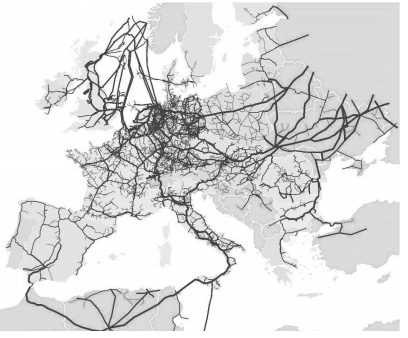
\includegraphics[width=0.5\textwidth]{res/h25.png}
\caption{Mạng lưới đường ống khí đốt ở Châu Âu.}
\label{fig:h25}
\end{figure}\par
Nếu một người muốn giải thích sự phân phối một cách đơn giản, có một loại mạng phân phối đã được nghiên cứu khá tốt là mạng sông (river networks), mặc dù mạng sông chính xác hơn là một mạng thu thập thay vì là mạng phân phối. Trong một mạng sông, các cạnh là sông hoặc suối và giao điểm của chúng là các đỉnh. Giống mạng lưới đường bộ, không có kĩ thuật đặc biệt nào để thu thập dữ liệu về cấu trúc mạng sông. Công việc khảo sát đã được thực hiện bởi khảo sát viên và người vẽ bản đồ, tất cả những gì ta làm chỉ là sao chép kết quả từ bản đồ ra.
\begin{figure}[ht]
\centering
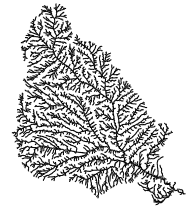
\includegraphics[width=0.5\textwidth]{res/h26.png}
\caption{Lưu vực thoát nước ở Loess Plateau: Mạng lưới sông suối trên Loess Plateau ở Sơn Tây tỉnh của Trung Quốc. Nhìn thấy được trong cấu trúc giống như cây của mạng là không có vòng lặp, vì vậy nước tại bất kỳ điểm nào trong mạng đều có một đường để thoát ra}
\label{fig:h26}
\end{figure}\par
